\documentclass[10pt,a4paper]{article}
\usepackage[utf8]{inputenc}
\usepackage[T1]{fontenc}
\usepackage{babel}
\babelprovide[import,main]{portuguese}
\usepackage{lmodern,amsmath,amssymb,booktabs,tabularx,array,graphicx}
\usepackage[margin=2cm]{geometry}
\usepackage{tikz}
\usetikzlibrary{arrows.meta,positioning}
\usepackage[hidelinks]{hyperref}
\usepackage{enumitem}
\setlist{nosep,leftmargin=*}
\setlength{\parindent}{1.1em}
\setlength{\parskip}{2.5pt}
\setlength{\emergencystretch}{2em}
\newcommand{\cod}[1]{\texttt{\detokenize{#1}}}
\newcommand{\Y}{\mathrm{Y}}
\title{Do simbólico à incerteza: infraestrutura digital básica\\nas escolas do Amazonas}
\author{\small Camila dos Santos Soares, Daniel Nunes Santos, José Eduardo,\\\small Nicoly Lima de Souza, Pedro Matheus Melo Pereira e Pedro Vinícius Díaz de Alencar\\[3pt]\small Fundamentos de Inteligência Artificial --- Prof. Edjard Mota}
\date{Novembro de 2026}
\begin{document}
\maketitle
\begin{abstract}
Este trabalho aplica seis abordagens de Inteligência Artificial a dados do Censo Escolar 2025, com recorte para escolas do Amazonas. A classificação identifica infraestrutura digital básica e a regressão estima equipamentos para alunos por sala. Implementamos árvore de decisão, regressões, cálculos de probabilidade, Naive Bayes, Expectation-Maximization (EM), rede Bayesiana e lógica fuzzy. A árvore atingiu 87,65\% de acurácia média em cinco folds. O Naive Bayes obteve 84,42\%, e a inclusão de um perfil obtido por EM reduziu o resultado para 83,34\% em uma divisão 70/30. A enumeração coincidiu com a eliminação de variáveis do pgmpy. O sistema fuzzy recebe as probabilidades da rede e fornece urgência de apoio interpretável. Discutimos desbalanceamento, limitações do DAG e diferenças entre interpretar decisões e melhorar a previsão.
\end{abstract}
\noindent\textbf{Palavras-chave:} Censo Escolar; árvore de decisão; redes Bayesianas; EM; lógica fuzzy.

\section{Problema, dados e preparação}
A pergunta principal é: \emph{a escola tem infraestrutura digital básica?} Adotamos um critério operacional, sem pretender avaliar toda a qualidade da escola. A classe $Y=1$ exige internet para alunos e pelo menos um tipo de equipamento para eles: desktop, computador portátil ou tablet. A internet informada não deve ser interpretada especificamente como conexão Wi-Fi. As demais escolas recebem $Y=0$.

A fonte registrada pela equipe é o arquivo \cod{Tabela_Escola_2025_V2.csv}, do INEP, com acesso em 29/10/2026 \cite{inep}. Filtramos Amazonas e situação de funcionamento igual a 1. A base de classificação contém 5.562 escolas: 4.555 da classe 0 (81,90\%) e 1.007 da classe 1 (18,10\%). O identificador \cod{CO_ENTIDADE} não participa do aprendizado. As colunas que definem o alvo também não entram como preditoras da classificação.

\begin{center}\small
\begin{tabular}{lll}\toprule
Símbolo & Coluna & Significado/códigos\\\midrule
$L$ & \cod{IN_LABORATORIO_INFORMATICA} & Laboratório, 0/1\\
$B$ & \cod{IN_BIBLIOTECA} & Biblioteca, 0/1\\
LOC & \cod{TP_LOCALIZACAO} & 1 urbana; 2 rural\\
DEP & \cod{TP_DEPENDENCIA} & 1 federal; 2 estadual; 3 municipal; 4 privada\\
$G$ & \cod{IN_ENERGIA_GERADOR_FOSSIL} & Gerador a combustível fóssil, 0/1\\\bottomrule
\end{tabular}\end{center}

O gerador da primeira base remove ausentes nas pistas e trata ausentes nas colunas do alvo como zero. Essa última decisão exige cuidado: não informado não significa necessariamente inexistente. O registro de execução fornecido pela equipe informa ausência de vazios no recorte utilizado; os CSVs finais também não têm ausentes. A fonte bruta e o dicionário devem ser preservados pela equipe para rastreabilidade.

A segunda base tem 5.526 escolas e alvo contínuo
\[
D=\frac{\text{QT\_DESKTOP\_ALUNO}+\text{QT\_COMP\_PORTATIL\_ALUNO}+\text{QT\_TABLET\_ALUNO}}{\text{QT\_SALAS\_UTILIZADAS}}.
\]
Seu gerador trata o código 88888 como ausente nas quantidades usadas, remove ausentes e restringe escolas a até 60 salas. Esse limite é uma escolha de limpeza, não uma regra do domínio. Os arquivos tratados permitem executar os notebooks sem baixar o microdado nacional. O escopo implementado usa dados do INEP, sem junção com IBGE.

\newpage
\section{Etapa 1: árvore, entropia e limites da lógica}
Implementamos LEARN-DECISION-TREE, com divisões por valores categóricos e escolha do maior ganho de informação \cite{russell}. Folhas puras retornam a classe; sem atributos ou ao atingir a profundidade máxima, usamos a maioria. Um valor não observado no treino recebe a classe majoritária do nó. Comparamos a implementação com \emph{DecisionTreeClassifier}, usando codificação one-hot para o sklearn.

\subsection{Cálculos dos três primeiros níveis}
Contamos a raiz como nível 1, seus filhos como nível 2 e os netos como nível 3. Para duas classes, definimos $h(p)=-p\log_2p-(1-p)\log_2(1-p)$, com $h(0)=h(1)=0$. Assim,
\[
H(S)=h\!\left(\frac{n_1}{N}\right),\qquad
GI(S,A)=H(S)-\sum_v\frac{N_v}{N}h\!\left(\frac{n_{1,v}}{N_v}\right).
\]
Na raiz, $H=h(1007/5562)=0,68237$ bit. O laboratório separa 4.607 escolas (369 positivas) de 955 (638 positivas). A entropia ponderada é $0,49084$; portanto, $GI=0,68237-0,49084=0,19153$. A tabela apresenta as frações de cada ramo.
Os ganhos dos outros candidatos na raiz são: biblioteca 0,09893; localização 0,09528; dependência 0,04378; gerador 0,00878. Portanto, laboratório é escolhido. A tabela mostra as substituições numéricas de cada divisão dos três níveis. Subtrai-se a quarta coluna da terceira para obter a última.

\begin{center}\scriptsize
\setlength{\tabcolsep}{3pt}\renewcommand{\arraystretch}{1.6}
\begin{tabular}{llccc}\toprule
Condição do nó & Atributo & Entropia do nó & Entropia ponderada dos filhos & Ganho\\\midrule
Raiz & L & $h(1007/5562)$ & $\frac{4607h\!\left(\frac{369}{4607}\right)+955h\!\left(\frac{638}{955}\right)}{5562}$ & 0.19153 \\
L=0 & LOC & $h(369/4607)$ & $\frac{1107h\!\left(\frac{181}{1107}\right)+3500h\!\left(\frac{188}{3500}\right)}{4607}$ & 0.01869 \\
L=0, LOC=1 & DEP & $h(181/1107)$ & $\frac{2h\!\left(\frac{1}{2}\right)+220h\!\left(\frac{41}{220}\right)+608h\!\left(\frac{76}{608}\right)+277h\!\left(\frac{63}{277}\right)}{1107}$ & 0.01084 \\
L=0, LOC=2 & DEP & $h(188/3500)$ & $\frac{137h\!\left(\frac{2}{137}\right)+3360h\!\left(\frac{185}{3360}\right)+3h\!\left(\frac{1}{3}\right)}{3500}$ & 0.00167 \\
L=1 & DEP & $h(638/955)$ & $\frac{17h\!\left(\frac{17}{17}\right)+401h\!\left(\frac{212}{401}\right)+413h\!\left(\frac{314}{413}\right)+124h\!\left(\frac{95}{124}\right)}{955}$ & 0.05249 \\
L=1, DEP=2 & G & $h(212/401)$ & $\frac{400h\!\left(\frac{212}{400}\right)+1h\!\left(\frac{0}{1}\right)}{401}$ & 0.00271 \\
L=1, DEP=3 & LOC & $h(314/413)$ & $\frac{285h\!\left(\frac{235}{285}\right)+128h\!\left(\frac{79}{128}\right)}{413}$ & 0.03468 \\
L=1, DEP=4 & G & $h(95/124)$ & $\frac{116h\!\left(\frac{87}{116}\right)+8h\!\left(\frac{8}{8}\right)}{124}$ & 0.02576 \\

\bottomrule\end{tabular}\end{center}
O ramo $L=1$, DEP=1 contém 17 escolas, todas positivas; sua entropia é zero e não requer nova divisão. Ramos sem exemplos não contribuem para a soma ponderada. As expressões permitem refazer os cálculos com calculadora; o histórico da implementação foi usado para conferir contagens e resultados.

\subsection{Validação e monotonicidade}
Com profundidade 3, a validação estratificada 5-fold obteve $87,65\%\pm0,32$ ponto percentual para a árvore própria e 87,67\% para o sklearn com entropia. Prever sempre a maioria alcança 81,90\%. A árvore sem limite obteve 87,52\%, sem vantagem observada. O ID3 tem divisões multirramos, enquanto o sklearn usa divisões binárias; profundidades iguais não garantem estruturas equivalentes.

Na lógica clássica, monotonicidade significa que acrescentar premissas a uma base não retira consequências que já eram deriváveis. A aprendizagem por exemplos funciona de outra maneira: o modelo é uma hipótese estimada a partir de uma amostra e pode ser revisto quando chegam observações novas. Uma previsão da árvore não é uma verdade universal demonstrada sobre todas as escolas.

Por exemplo, considere uma folha com duas escolas da classe 0 e uma da classe 1. A maioria leva à previsão 0. Se incluirmos duas novas escolas da classe 1 com as mesmas pistas e treinarmos novamente, a folha passa a ter duas negativas e três positivas. Sua previsão muda para 1, inclusive para uma escola que anteriormente recebia 0. Novos exemplos também podem alterar os ganhos de informação e a estrutura dos ramos.

Isso não contradiz a monotonicidade da dedução clássica: são operações diferentes. A dedução preserva consequências das premissas; a indução modifica a hipótese para acomodar a evidência disponível. Uma regra universal como ``toda escola com laboratório tem infraestrutura digital básica'' também é inadequada: há 317 contraexemplos entre as 955 escolas com laboratório. A árvore produz uma decisão baseada em frequências, sujeita a erro e revisão. Por isso avaliamos escolas fora do treino e tratamos as regras como padrões dos dados, não como garantias.

\newpage
\section{Etapa 2: aprendizado linear}
Para prever $D$, usamos internet para alunos, laboratório, internet para aprendizagem, quantidade de TVs, quantidade de equipamentos multimídia e lousa digital. São informações de infraestrutura; não incluímos diretamente as quantidades de aparelhos que compõem o numerador do alvo.

Na regressão univariada, calculamos a reta pela fórmula fechada:
\[
\hat D=\theta_0+\theta_1x,\quad
\theta_1=\frac{\sum_i(x_i-\bar x)(D_i-\bar D)}{\sum_i(x_i-\bar x)^2},\quad
\theta_0=\bar D-\theta_1\bar x.
\]
A preditora padrão é internet para alunos, definida antes de avaliar o teste pela associação interpretável entre conectividade e disponibilidade de equipamentos. A reta obtida é $\hat D=0,2776+2,2107x$, com $R^2=0,2372$ no teste. A avaliação não seleciona a variável. Essa correção substitui o procedimento anterior, que destacava o maior resultado entre variáveis usando o próprio teste.

Na multivariada, minimizamos $J(\theta)=\|X\theta-D\|^2/(2m)$ por
$\theta\leftarrow\theta-\alpha X^T(X\theta-D)/m$. Adicionamos uma coluna de 1 para o intercepto e padronizamos preditoras com média e desvio do treino. Com $\alpha=0,1$, a execução convergiu em 163 iterações. A comparação com \emph{LinearRegression} usou as mesmas escolas e produziu o mesmo $R^2$ arredondado.

No Ridge, acrescentamos $\lambda\sum_{j\geq1}\theta_j^2/(2m)$ ao custo, sem penalizar o intercepto. A escolha de $\lambda$ foi feita por cinco folds somente no treino. O valor selecionado foi aproximadamente 77,43. O gradiente regularizado foi conferido contra a solução fechada; a diferença máxima nos coeficientes ficou abaixo de $6\times10^{-7}$ nos valores testados. A penalização controla a magnitude global dos coeficientes; não exige que cada coeficiente individual diminua monotonicamente em todo trecho do caminho.

\begin{center}\small
\begin{tabular}{lrr}\toprule
Modelo & $R^2$ teste & MSE teste\\\midrule
Univariada (internet para alunos) & 0,2372 & 2,0311\\
Multivariada por gradiente & 0,3228 & 1,8030\\
Ridge, $\lambda$ escolhido por CV & 0,3237 & 1,8006\\\bottomrule
\end{tabular}\end{center}
\begin{center}
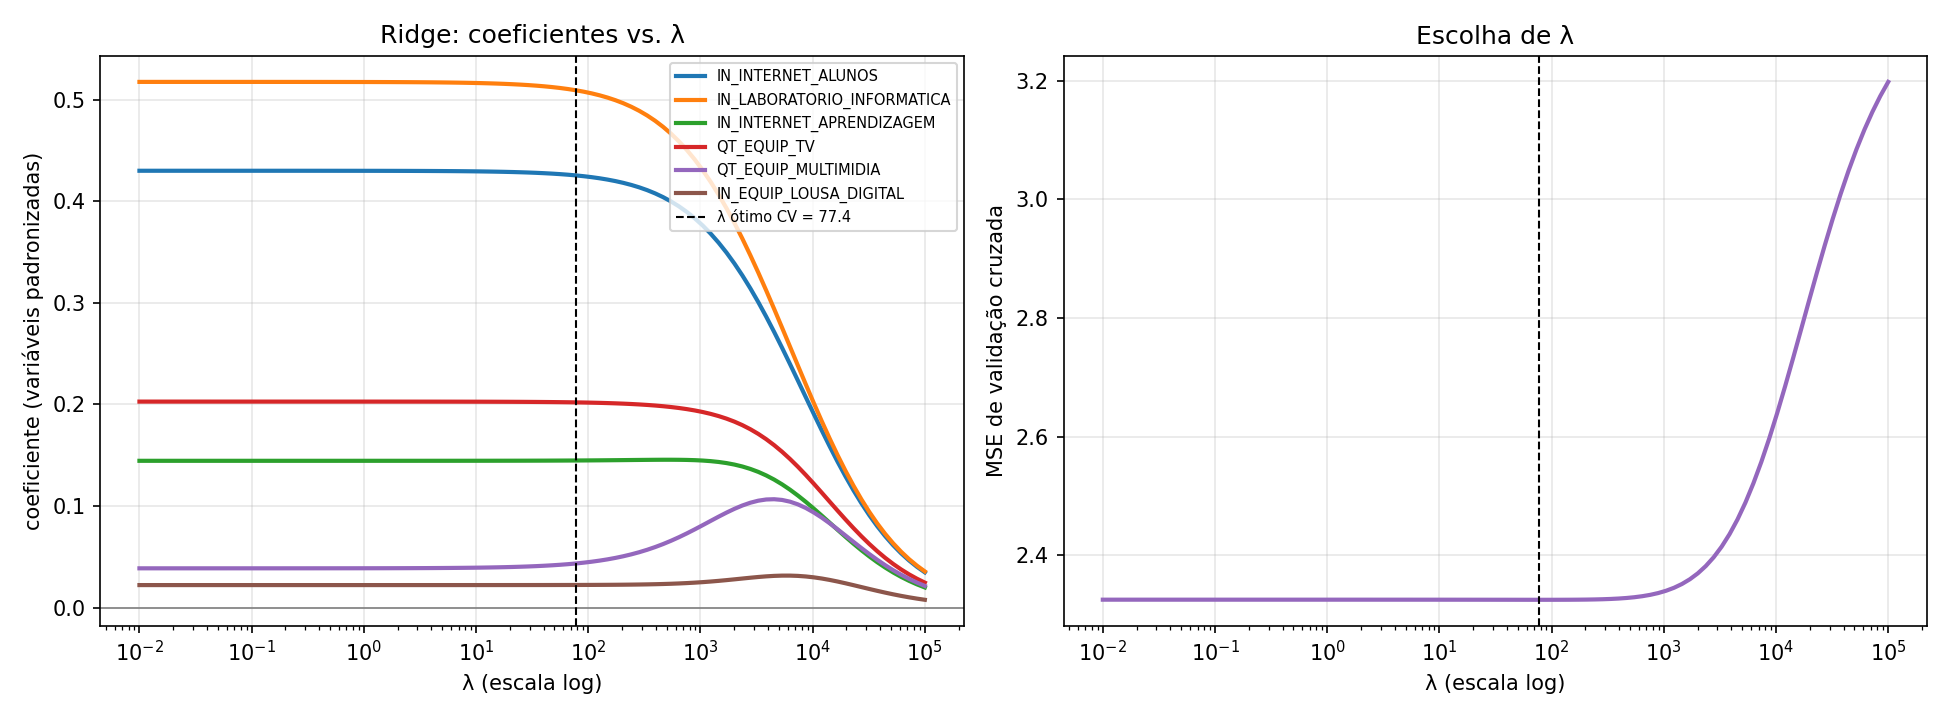
\includegraphics[width=.91\linewidth]{figuras/ridge_coeficientes.png}
\end{center}
\noindent\small Figura 1: caminho dos coeficientes e escolha de $\lambda$ por validação no treino.\normalsize

A logística retorna ao alvo binário da Etapa 1. Implementamos sigmoide, entropia cruzada e gradiente, com $P(Y=1\mid x)=1/(1+e^{-x^T\theta})$. Dependência administrativa usa variáveis indicadoras; o identificador é excluído. A comparação com \emph{LogisticRegression}, praticamente sem regularização, apresentou diferença máxima de coeficientes de cerca de 0,0018.

Em uma divisão estratificada 80/20, com limiar 0,5, a logística obteve 88,40\% de acurácia, precisão 76,87\%, recall 51,24\%, F1 61,49\% e AUC 0,8358. A matriz de confusão foi $\left[\begin{smallmatrix}880&31\\98&103\end{smallmatrix}\right]$. Assim, quase metade das escolas positivas não foi identificada. O baixo $R^2$ das regressões e o recall limitado da logística mostram que essas pistas não resumem todos os fatores de informatização. O pequeno ganho de Ridge deve ser apresentado sem exagero.

\newpage
\section{Etapa 3: probabilidade}
O experimento é escolher uma escola uniformemente entre as 5.562 linhas. Os eventos são definidos pelas características observadas. Satisfazemos não negatividade, $P(\Omega)=1$ e aditividade para eventos disjuntos. As quatro combinações de laboratório e biblioteca são disjuntas e cobrem a base:
\begin{center}\small
\begin{tabular}{crr}\toprule
Evento $(L,B)$ & Contagem & Probabilidade\\\midrule
$(0,0)$ & 3994 & 0,71809\\
$(0,1)$ & 613 & 0,11021\\
$(1,0)$ & 213 & 0,03830\\
$(1,1)$ & 742 & 0,13341\\\bottomrule
\end{tabular}\end{center}
As probabilidades somam 1 antes de arredondar. Temos $P(L=1)=955/5562=0,17170$ e $P(B=1)=1355/5562=0,24362$. As condicionais usam denominadores distintos: $P(B=1\mid L=1)=742/955=77,70\%$ e $P(L=1\mid B=1)=742/1355=54,76\%$.

A regra da cadeia para três variáveis é verificada por
\[
P(Y=1,L=1,B=1)=\frac{1007}{5562}\frac{638}{1007}\frac{496}{638}
=\frac{496}{5562}=8,9177\%.
\]
Por Bayes, $P(Y=1\mid L=1)=P(L=1\mid Y=1)P(Y=1)/P(L=1)=638/955=66,81\%$. Trata-se de uma inferência diagnóstica a partir da pista; não mede o efeito causal de instalar um laboratório. Para $Y=0$, $P(L=1,B=1\mid Y)=5,40\%$, mas o produto das marginais condicionais é 1,14\%. Para $Y=1$, os valores são 49,26\% e 38,32\%. Logo, não há independência condicional exata na distribuição empírica.

Na lógica de primeira ordem clássica, a afirmação sobre uma escola é verdadeira ou falsa em uma interpretação. Uma chance de 70\% exige uma distribuição, que não é expressa apenas pelo valor de verdade de um predicado. A probabilidade permite representar frequências e incerteza, em vez de assumir uma regra universal sem exceções.

\section{Etapa 4: aprendizado probabilístico e EM}
Dividimos a base em 70\% de treino e 30\% de teste, com \cod{random_state=42}. Essa divisão não é estratificada. Entre 3.893 escolas de treino, 725 são positivas. Para uma Bernoulli, $\hat\theta_{MLE}=s/n=0,1862$. Com prior Beta$(2,2)$, o máximo a posteriori é
\[
\hat\theta_{MAP}=\frac{s+2-1}{n+2+2-2}=\frac{726}{3895}=0,1864.
\]
O Naive Bayes próprio estima $P(Y)$ e $P(X_j\mid Y)$ por contagens com suavização de Laplace. Na previsão, soma logaritmos para evitar produtos muito pequenos. A independência condicional é uma aproximação, já contrariada por laboratório e biblioteca na etapa anterior.

Para inferir uma variável oculta $Z\in\{0,1\}$, ajustamos uma mistura de Bernoulli sobre laboratório, biblioteca e gerador, apenas no treino. No passo E, calculamos responsabilidades $r_{ik}=P(Z=k\mid x_i)$. No passo M, atualizamos $\pi_k=\sum_i r_{ik}/n$ e $p_{kj}=\sum_i r_{ik}x_{ij}/\sum_i r_{ik}$. Monitoramos $\ell=\sum_i\log\sum_k\pi_kP(x_i\mid Z=k)$ e paramos quando a mudança média por escola fica abaixo de $10^{-7}$, com limite de 500 avaliações.

A curva cresceu até a avaliação 105. Um perfil, de peso 0,294, apresentou probabilidades de 0,596 para laboratório, 0,777 para biblioteca e 0,030 para gerador. O outro, de peso 0,706, apresentou aproximadamente 0,000, 0,025 e 0,162; o zero exibido é arredondamento. O gráfico está no notebook da etapa.

No mesmo teste de 1.669 escolas, NB puro obteve 84,42\% e NB com o perfil mais provável do EM obteve 83,34\%. O perfil resume pistas já utilizadas; sua inclusão pode reforçar informação dependente. Maior verossimilhança da mistura não garante melhor classificação. Mantemos a piora observada e não interpretamos perfis como categorias oficiais de escolas.
\begin{center}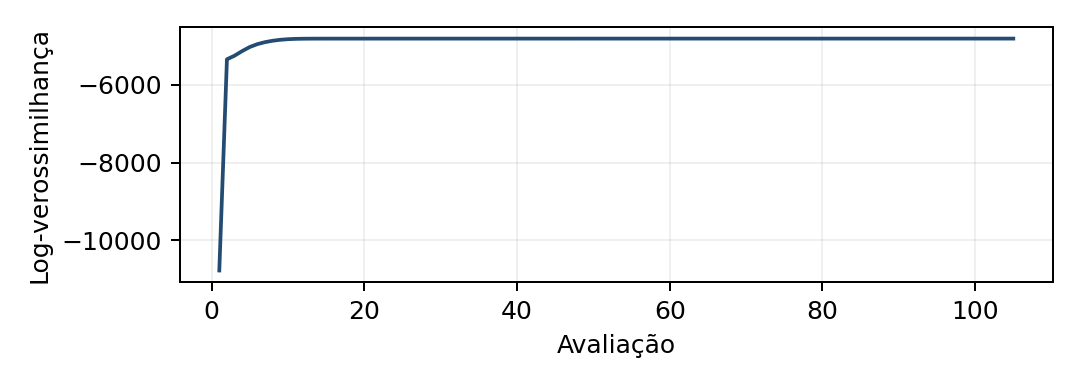
\includegraphics[width=.60\linewidth,height=3.3cm,keepaspectratio]{figuras/em_convergencia.png}\\{\small Log-verossimilhança da mistura Bernoulli no treino.}\end{center}

\newpage
\section{Etapa 5: redes Bayesianas}
Modelamos seis variáveis por um DAG. As arestas indicam dependências plausíveis, sem comprovação causal: LOC$\to$DEP descreve a distribuição das redes por localização; LOC$\to G$ relaciona localização e uso de gerador; DEP$\to L$ e DEP$\to B$ representam diferenças de investimento; $G\to L$ e $G\to Y$ representam associação com a disponibilidade de energia; $L\to Y$ e $B\to Y$ associam infraestrutura física ao alvo.
\begin{center}
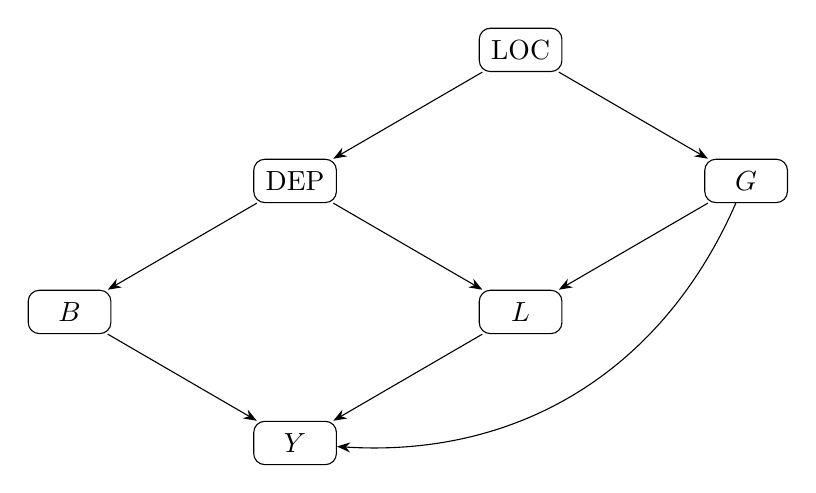
\begin{tikzpicture}[>=Stealth,node distance=1.1cm and 1.8cm,every node/.style={draw,rounded corners,minimum width=1.05cm,minimum height=.55cm}]
\node (loc) {LOC}; \node (dep) [below left=of loc] {DEP}; \node (g) [below right=of loc] {$G$};
\node (b) [below left=of dep] {$B$}; \node (l) [below right=of dep] {$L$}; \node (y) [below right=of b] {$Y$};
\draw[->] (loc)--(dep);\draw[->] (loc)--(g);\draw[->] (dep)--(b);\draw[->] (dep)--(l);\draw[->] (g)--(l);\draw[->] (g) to[bend left=35] (y);\draw[->] (b)--(y);\draw[->] (l)--(y);
\end{tikzpicture}
\end{center}
\noindent\small Figura 2: DAG efetivamente implementado na versão analisada.\normalsize

As tabelas condicionais (CPTs) são estimadas por
$P(X=x\mid c)=[N(x,c)+1]/[N(c)+|X|]$. Isso evita zeros em combinações raras. A enumeração própria soma o produto das CPTs sobre variáveis ocultas e normaliza. Conferimos 76 consultas contra a marginalização da conjunta, cuja soma é 1; a maior diferença foi $2,2\times10^{-16}$.

Também comparamos com \emph{VariableElimination} do pgmpy: primeiro com as mesmas CPTs, depois com CPTs estimadas pela biblioteca usando prior K2. Na execução de verificação, a diferença máxima das consultas foi $1,11\times10^{-16}$, e a diferença das CPTs foi zero. Essa concordância valida a inferência para o modelo, não a fidelidade do modelo ao mundo real.

\begin{center}\small
\begin{tabular}{lrr}\toprule
Consulta & Rede & Frequência empírica\\\midrule
$P(Y=1)$ & 0,1890 & 0,1810\\
$P(Y=1\mid LOC=2)$ & 0,1484 & 0,0780\\
$P(Y=1\mid L=1)$ & 0,6643 & 0,6681\\
$P(LOC=2\mid Y=1)$ & 0,5175 & 0,2840\\\bottomrule
\end{tabular}\end{center}

\subsection{d-separação e colisor}
No grafo, $B\perp L\mid DEP$: observar DEP bloqueia as bifurcações relevantes, enquanto os caminhos por $Y$ contêm colisor não observado. Ao observar também $Y$, o caminho $B\to Y\leftarrow L$ abre. A segunda independência é $DEP\perp G\mid LOC$; observar o colisor $L$ abre $DEP\to L\leftarrow G$. Conferimos bloqueios por caminhos e por moralização do grafo ancestral.

Um exemplo numérico fixa DEP=3. Sem observar $Y$, a rede dá $P(L=1)=0,0947$ tanto com $B=0$ quanto com $B=1$. Observando $Y=1$, os valores mudam de aproximadamente 0,52 para 0,26: a biblioteca ajuda a explicar o resultado e reduz a probabilidade de laboratório no modelo. Nos dados, biblioteca e laboratório continuam associados positivamente; o exemplo demonstra o mecanismo do grafo, não um efeito causal constatado.

Os testes empíricos rejeitam as duas independências, com efeitos diferentes: informação mútua condicional de aproximadamente 0,119 bit para biblioteca/laboratório e 0,010 bit para dependência/gerador. Estratos pequenos limitam o qui-quadrado. A falta de LOC$\to Y$ ajuda a explicar o erro nas consultas rurais. Avaliar essa aresta e $B\to L$ é uma melhoria futura, que exige nova validação.

\subsection{Economia de parâmetros}
A conjunta precisa de $2\cdot4\cdot2\cdot2\cdot2\cdot2-1=127$ parâmetros livres. A rede precisa de $1+6+2+4+8+8=29$, considerando cada nó e as configurações dos pais: economia de 98, ou 77,2\%. As duas arestas propostas elevariam o total para 45. A economia reduz complexidade, mas introduz viés quando as independências assumidas não representam bem os dados.

\newpage
\section{Etapa 6: lógica fuzzy e integração}
O sistema Mamdani usa \emph{scikit-fuzzy}. A primeira entrada é risco $r=P(Y=0\mid e)$, calculado pela enumeração da Etapa 5. A segunda é suporte amostral, denominado confiança: $c=\min(N_e,100)$, em que $N_e$ conta escolas do treino com a mesma evidência. A saída é urgência de apoio, de 0 a 100. Essa confiança é uma heurística, não um intervalo estatístico nem garantia de acerto.

Os vértices das funções de pertinência triangulares são apresentados abaixo, separados por ponto e vírgula:
\begin{center}\small
\begin{tabular}{llll}\toprule
Variável & Baixo/baixa & Médio/média & Alto/alta\\\midrule
Risco & $[0;0;0,5]$ & $[0,25;0,5;0,75]$ & $[0,5;1;1]$\\
Confiança & $[0;0;100]$ & --- & $[0;100;100]$\\
Urgência & $[0;0;50]$ & $[25;50;75]$ & $[50;100;100]$\\\bottomrule
\end{tabular}\end{center}
Os conjuntos cobrem os universos; suas pertinências não precisam somar 1 e, no risco e na urgência, essa soma varia de 0,5 a 1. As três regras são:
\begin{enumerate}
\item Se risco é alto \textbf{e} confiança é alta, então urgência é alta.
\item Se risco é médio \textbf{ou} confiança é baixa, então urgência é média.
\item Se risco é baixo, então urgência é baixa.
\end{enumerate}
Usamos mínimo para E, máximo para OU e agregação, e centroide para defuzzificação \cite{zadeh,hullermeier}. A saída recebe o termo com maior pertinência. Por exemplo, escolas urbanas estaduais sem gerador têm $N=586$ e $P(Y=1)=0,426$ na rede ajustada à base completa. O risco 0,574 ativa a regra média em aproximadamente 0,703 e a alta em 0,149, resultando em urgência 55,45, de rótulo médio.

\begin{center}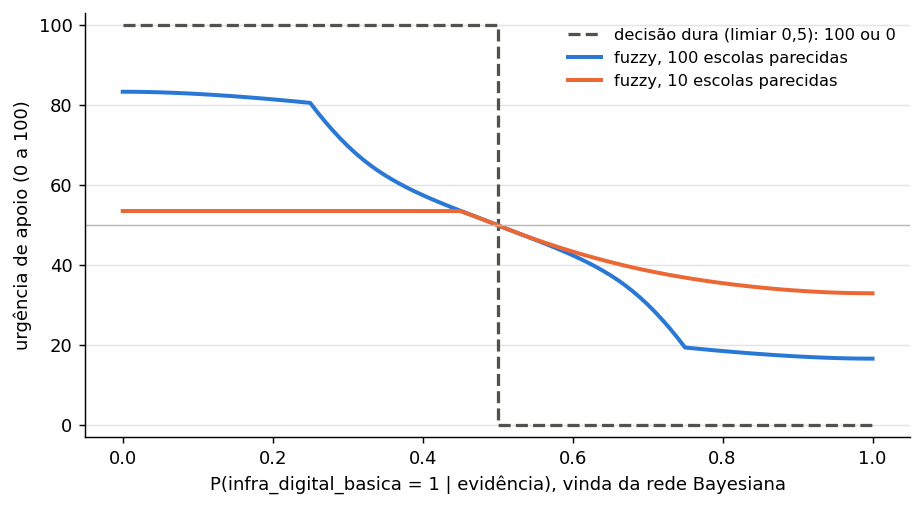
\includegraphics[width=.75\linewidth]{figuras/etapa6_curva.png}\end{center}
\noindent\small Figura 3: decisão dura e urgência fuzzy, variando a probabilidade e o suporte.\normalsize

Na avaliação 5-fold estratificada, CPTs e contagens vêm somente do treino. Com evidência LOC, DEP e $G$, fuzzy e limiar duro concordaram em 100\% das escolas, com acurácia 82,29\% e recall positivo de apenas 2,28\%. A AUC para falta de infraestrutura foi 0,511 na decisão dura, 0,666 na probabilidade da rede e 0,656 na urgência. Portanto, o fuzzy preserva parte da ordenação perdida pelo limiar e oferece rótulos, mas não supera a probabilidade original em discriminação.

Com evidência $G,L,B$, a acurácia foi 87,67\% para as duas decisões; a AUC da rede foi 0,816 e a fuzzy, 0,815. O aumento depende da evidência adicional, não apenas do fuzzy. Os triângulos e o limite de 100 escolas foram escolhas da equipe. Urgência 83 não significa 83\% de chance. O centroide produz, neste sistema, extremos próximos de 17 e 83. A falta de dados puxa a decisão para o meio; um gestor ainda precisa validar as regras e as prioridades.

\newpage
\section{Integração, discussão e reprodução}
\begin{center}
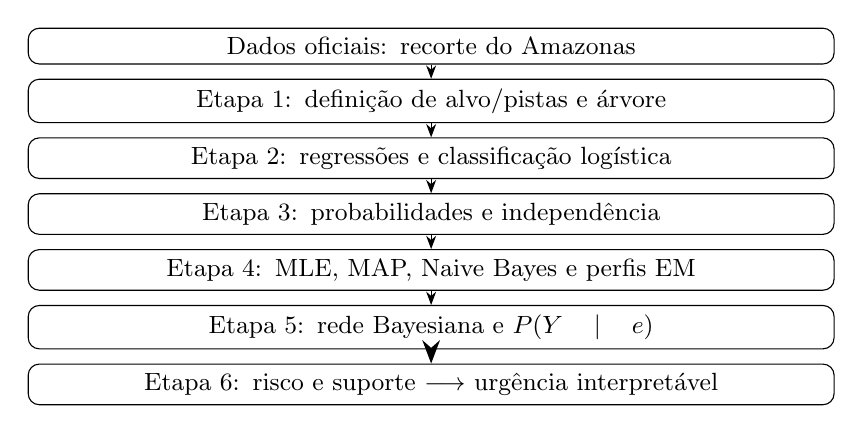
\begin{tikzpicture}[>=Stealth,node distance=.18cm,every node/.style={draw,rounded corners,align=center,text width=10cm,minimum height=.42cm,font=\small}]
\node (d) {Dados oficiais: recorte do Amazonas};
\node (a) [below=of d] {Etapa 1: definição de alvo/pistas e árvore};
\node (b) [below=of a] {Etapa 2: regressões e classificação logística};
\node (c) [below=of b] {Etapa 3: probabilidades e independência};
\node (e) [below=of c] {Etapa 4: MLE, MAP, Naive Bayes e perfis EM};
\node (f) [below=of e] {Etapa 5: rede Bayesiana e $P(Y\mid e)$};
\node (g) [below=of f] {Etapa 6: risco e suporte $\longrightarrow$ urgência interpretável};
\draw[->,dashed] (d)--(a);\draw[->,dashed] (a)--(b);\draw[->,dashed] (b)--(c);\draw[->,dashed] (c)--(e);\draw[->,dashed] (e)--(f);\draw[->,very thick] (f)--(g);
\end{tikzpicture}
\end{center}
\noindent\small Figura 4: sequência metodológica (tracejada) e transferência de probabilidades 5--6 (contínua). A integração adicional 1/4--6 é descrita no texto.\normalsize

O CSV, o alvo e as pistas da Etapa 1 são reaproveitados nas Etapas 3--6. A integração operacional implementada é 5$\to$6: \cod{fuzzy.py} importa a enumeração e calcula suas entradas. O uso de suavização também relaciona as etapas probabilísticas: em uma linha Bernoulli, Laplace coincide com o MAP Beta$(2,2)$; para mais categorias, a formulação correspondente usa Dirichlet.

\textbf{Integração operacional adicional.} O script \cod{integracao.py} usa todas as cinco pistas em uma divisão estratificada 70/30. Árvore, NB e CPTs são ajustados apenas no treino. A probabilidade do NB modula a confiança fuzzy por $\min(N_e,100)(1-|P_{NB}-P_{rede}|)$. A decisão da árvore encaminha a ação final para revisão quando diverge da classe da rede. Essa regra é uma heurística explícita, não confiança estatística. A demonstração não substitui os resultados anteriores em cinco folds nem comprova ganho de acurácia.

Os resultados mostram diferentes compromissos. A árvore gera regras simples; a regressão quantifica associações, com poder explicativo limitado; o NB simplifica dependências e o EM identifica perfis, sem ganho de acurácia observado. A rede representa dependências explicitamente e permite consultas, mas seu DAG produz viés. O fuzzy organiza uma decisão legível e suave, sem corrigir erros das probabilidades de entrada.

As métricas não formam um ranking único: árvore e fuzzy usam cinco folds, NB usa 70/30 e logística usa 80/20; algumas comparações também mudam as evidências. Uma comparação conclusiva entre algoritmos requer mesmas partições e mesmas informações disponíveis. O desbalanceamento exige considerar recall e F1, além de acurácia. Também não extrapolamos automaticamente os resultados do Amazonas para outros estados ou anos.

\subsection{Reprodução e versão dos resultados}
Este artigo documenta a revisão de 07/11/2026, baseada no commit \cod{2a7676f}, com seleção univariada corrigida, do repositório da equipe\footnote{\url{https://github.com/pwtheus/pipeline-ia-simbolico-incerteza}}. Instalam-se as dependências de \cod{requirements.txt}, seleciona-se o ambiente Python no VS Code e executam-se \cod{etapa1.ipynb} a \cod{etapa6.ipynb}, a partir da raiz. As divisões usam sementes fixas; há também semente 0 no sklearn e na CV interna do Ridge, além de 42 nas principais divisões.

A execução de verificação percorreu as células em processos Python separados, com Python 3.12, NumPy 2.3.5, pandas 2.2.3, scikit-learn 1.8.0, pgmpy 1.1.2 e scikit-fuzzy 0.5.0. As seis etapas concluíram sem exceções. Essa verificação não substitui a execução e gravação dos notebooks no ambiente da equipe. Alterações posteriores de dados, modelos ou divisão exigem atualizar números, gráficos e conclusões deste artigo.

\begin{thebibliography}{9}\small
\bibitem{russell} RUSSELL, S.; NORVIG, P. \emph{Artificial Intelligence: A Modern Approach}. 4. ed. Pearson, 2020.
\bibitem{zadeh} ZADEH, L. A. Fuzzy sets. \emph{Information and Control}, v. 8, n. 3, p. 338--353, 1965.
\bibitem{hullermeier} HÜLLERMEIER, E. Fuzzy machine learning and data mining. \emph{WIREs Data Mining and Knowledge Discovery}, v. 1, n. 4, p. 269--283, 2011.
\bibitem{inep} INEP. \emph{Censo Escolar 2025: Tabela Escola, versão V2}. Portal de dados abertos: \url{https://www.gov.br/inep/pt-br/acesso-a-informacao/dados-abertos}. Acesso registrado pela equipe: 29 out. 2026.
\end{thebibliography}

\newpage
\appendix
\small
\section{Uso de IA e registro de prompts}
Utilizamos assistentes de IA como apoio à organização, geração/revisão de código e explicação dos métodos. Os registros abaixo são uma seleção, não um histórico integral. \textbf{Fornecido} indica mensagem ou síntese enviada por integrantes; \textbf{reconstruído} indica uma formulação representativa preparada posteriormente para documentar o tipo de apoio, sem afirmar que foi digitada literalmente. Os registros da Etapa 1 informam uso do Claude. Este artigo e sua revisão também tiveram apoio do ChatGPT.

\subsection*{A.1 Registros fornecidos: definição do problema e Etapa 1}
\begin{enumerate}[label=\arabic*.]
\item \textbf{Pergunta e plano.} ``O domínio é educação, me dê sugestões que podemos buscar responder, porque através da pergunta podemos definir os atributos. Eu vou mandar a planilha com todas as colunas.'' Depois: ``Objetivo agora é fazer a primeira etapa.'' O apoio organizou as tarefas e sugeriu perguntas; a disponibilidade de colunas levou à escolha de infraestrutura.
\item \textbf{Alvo e pistas.} ``A escola se adequa a padrões modernos de informatização? Variáveis: laboratório de informática, biblioteca, localização, tipo de dependência, gerador de energia elétrica.'' O diálogo refinou a pergunta para infraestrutura digital básica e distinguiu pistas, alvo e identificador. Foram consultadas imagens do dicionário para conferir códigos.
\item \textbf{Definição operacional.} ``Para a Etapa 1 pode ser `a escola tem infraestrutura digital básica?', considerando que sim se tiver wifi e pelo menos um aparelho para os alunos.'' O resultado foi ajustado para internet para alunos, sem afirmar que é Wi-Fi, e pelo menos um indicador de aparelho. O script gerou o CSV; o registro da equipe informa 5.562 linhas e distribuição 4.555/1.007.
\item \textbf{Cálculo e revisão.} ``Por que estamos fazendo isso? O que essa tabela cruzada traz para a Etapa 1?''; ``Qual é a fórmula que a pessoa precisa saber?''; ``Meu amigo mandou isso, é coerente com o que você está fazendo?'' Também foi enviado o código da árvore para revisão. Foram explicados entropia e ganho, conferidos números e relacionada a implementação ao pseudocódigo.
\end{enumerate}

\subsection*{A.2 Registros fornecidos: Etapas 2 e 5}
\textbf{Etapa 2.} ``Estou fazendo um trabalho sobre Aprendizagem de Máquina, mais especificamente sobre Aprendizado Linear. Tenho de filtrar uma base de dados, escolhendo uma variável-alvo e variáveis preditivas. O tema é informatização da escola.'' Em seguida foi solicitada uma razão entre variáveis e escolhida a soma de desktops, portáteis e tablets dividida pelas salas utilizadas. O pedido final solicitou CSV e gerador, recorte Amazonas, tratamento dos problemas identificados e as seis preditoras descritas na Seção 3. O apoio resultou na preparação da base; os modelos foram conferidos com soluções fechadas e scikit-learn.

\textbf{Etapa 5.} ``Modelar dependências entre 4--6 variáveis do domínio usando uma rede Bayesiana, e usar inferência para responder consultas. Como devo preparar os dados para realizar as tarefas dessa parte? Posso utilizar os dados que utilizei na etapa 1 ou na etapa 2?'' Depois de fornecer a definição de \cod{infra_digital_basica}, foi pedido: ``Ajuste as arestas, se necessário, e desenhe o DAG.'' Outro pedido solicitou conferir economia de parâmetros, concordância com pgmpy e demonstração de colisor. O resultado foi confrontado com CPTs, enumeração, d-separação e contagem de parâmetros.

\subsection*{A.3 Prompts complementares reconstruídos}
\begin{enumerate}[label=\arabic*.]
\item \textbf{Validação e lógica:} ``Compare nossa árvore com o scikit-learn nas mesmas divisões, faça 5-fold estratificado e explique, com um exemplo simples, como novos dados podem alterar uma previsão. Não use apenas acurácia de treino.''
\item \textbf{Regressões:} ``Implemente fórmula fechada, gradiente descendente, Ridge e logística de forma simples. Padronize usando apenas o treino, escolha lambda por validação interna e compare com scikit-learn.''
\item \textbf{Probabilidade:} ``Use laboratório, biblioteca e a classe para calcular conjunta, marginais, condicionais, cadeia e Bayes. Confira as contagens e discuta independência e diferença entre associação e causalidade.''
\item \textbf{NB e EM:} ``Implemente MLE, MAP Beta(2,2), Naive Bayes do zero e EM Bernoulli com dois perfis. Ajuste somente no treino, mostre a log-verossimilhança e compare NB com e sem perfil, mesmo que o resultado piore.''
\item \textbf{Fuzzy:} ``Receba a probabilidade da Etapa 5 e o suporte amostral em um Mamdani com triângulos e 3--5 regras. Compare com limiar 0,5 e explique a urgência sem tratá-la como probabilidade.''
\item \textbf{Revisão e artigo:} ``Confira o repositório contra o enunciado, separe pendências importantes de melhorias opcionais e produza um artigo LaTeX com resultados verificados, limitações, cálculos e apêndice de uso de IA.''
\end{enumerate}
O código e os resultados, e não a resposta do chatbot, são a evidência do trabalho. As verificações descritas no artigo incluem contagens, equivalência numérica entre implementações e avaliação fora do treino. A equipe deve compreender os métodos e revisar o texto antes da entrega.
\end{document}
